% Draft. Generated with AI assistance under human direction; not yet reviewed by an analyst.
\documentclass[11pt]{article}

\usepackage[margin=1in]{geometry}
\usepackage{graphicx}
\usepackage{booktabs}
\usepackage{amsmath}
\usepackage{hyperref}
\usepackage{caption}

\title{Two-mode networks of culture elements, works, and definitions:\\
K\&K Index B, works and definition networks}
\author{Draft}
\date{\today}

\begin{document}
\maketitle

\begin{abstract}
We describe two two-mode networks built from the K\&K Index B of Kroeber and Kluckhohn's \emph{Culture: A Critical Review of Concepts and Definitions} (1952). In the \emph{definitions network}, Index B sub-elements are linked to the definition codes (A--G) under which they are indexed. In the \emph{works network}, sub-elements are linked to the authored works they cite. Both networks share the sub-element node set, which lets us compare how sub-elements are spread across definitions and across works. We report basic structure, degree distributions, nearest-neighbour degree, degree correlation, and modularity, then apply correspondence analysis and maximum spanning trees to each network. The analysis is descriptive. Several steps depend on decisions noted in the text.
\end{abstract}

\section{Data and networks}

The Index B sub-element matrix records, for each sub-element, the definition codes it is indexed under. We keep only the verified codes: 167 come from the K\&K Index A, and three (C-I-18a, D-II-16, E-17) come from the main text, with their basis in \texttt{data/kk-index-b-verified-extra-codes.csv}. The raw sub-element network already holds only these 170 codes, so the verified filter currently removes none. Sub-element names repeat across headings in the source, and the sub-element network treats same-named sub-elements as one node. No names repeat in the matrices used here, so the counts below are unaffected. The works network uses the same sub-element nodes, with ties to the works that cite each sub-element. Works are keyed by author and year, and a work can sit under several codes.

\section{Two-mode structure}

Table~\ref{tab:structure} reports the basic statistics. Edges are counted from the biadjacency matrices, and the two modes are counted separately, not from the total vertex count.

\begin{table}[ht]
\centering
\caption{Basic structure of the two networks (full networks, before any 2-core; isolated nodes included).}
\label{tab:structure}
\begin{tabular}{lrr}
\toprule
 & Definitions network & Works network \\
\midrule
Sub-element nodes & 472 & 472 \\
Second-mode nodes & 170 codes (5 isolated) & 133 works (4 isolated) \\
Edges & 1193 & 1165 \\
Density & 0.015 & 0.019 \\
Mean degree, sub-elements & 2.53 (range 1--36) & 2.47 (range 0--33) \\
Mean degree, second mode & 7.02 (range 0--25) & 8.76 (range 0--51) \\
\bottomrule
\end{tabular}
\end{table}

Degrees in the two modes count different things. A sub-element's degree is the number of codes (or works) it is linked to. A code's or work's degree is the number of sub-elements it contains. In each network the two degree sums equal the edge count.

\section{Degree distributions}

Figure~\ref{fig:degree} shows the degree distributions for each node set. Sub-elements in both networks are concentrated at low degree: the median is 1 in each network (interquartile range 1--2), so most sub-elements sit under one code or cite one or two works. The definition codes and works have more spread: among codes with at least one sub-element the median is 7 (interquartile range 4--10), and among works it is 8 (interquartile range 4--11), with a long tail. Each panel has its own axes, so the x-ranges differ across panels. Definition codes with no sub-elements are excluded from the figure; the four works with no sub-elements are shown at degree 0.

\begin{figure}[ht]
\centering
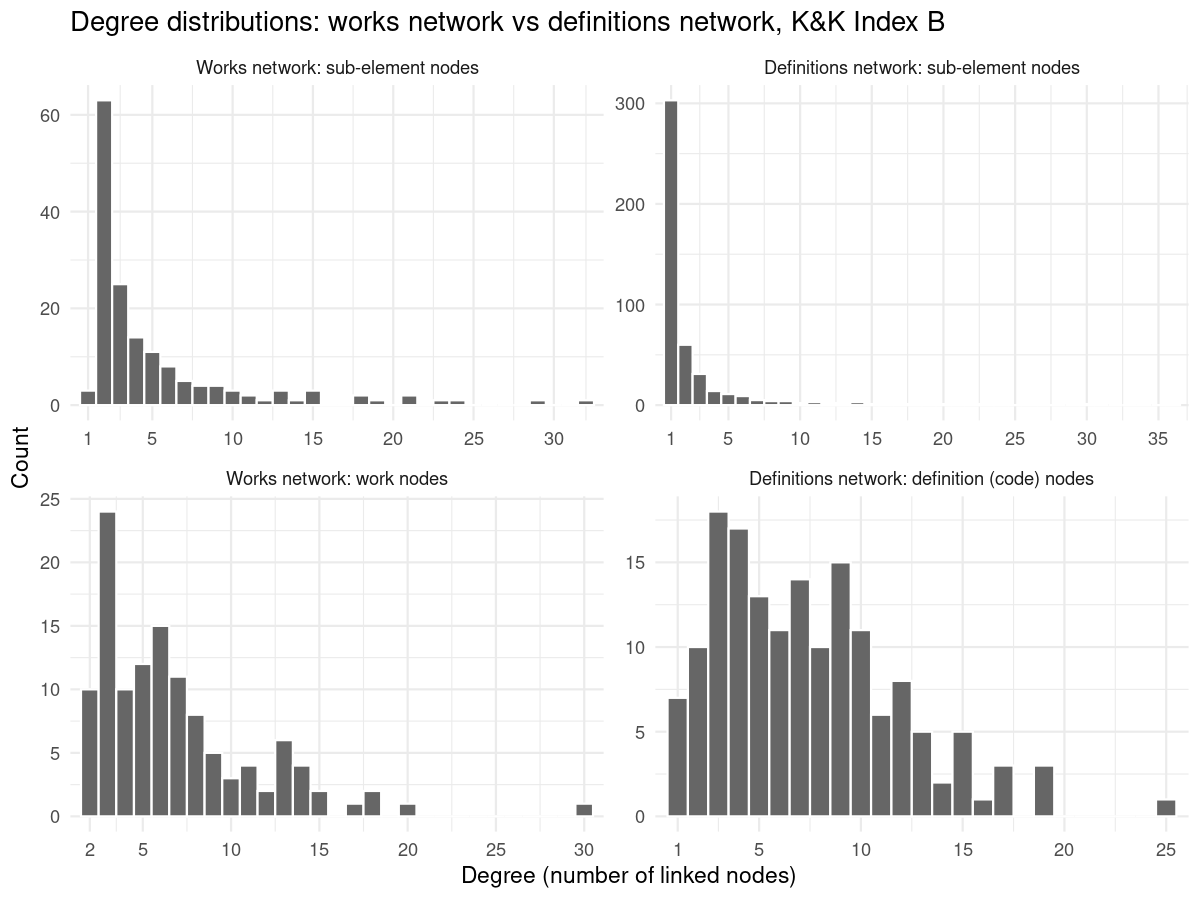
\includegraphics[width=\textwidth]{figures/kk-index-b/degree-works-definitions.png}
\caption{Degree distributions. Top row: sub-elements in the works network (left) and the definitions network (right). Bottom row: works (left) and definition codes (right).}
\label{fig:degree}
\end{figure}

\section{Degree centrality, nearest-neighbour degree, and degree correlation}

Degree centrality is the degree normalized by the size of the opposite mode. Average nearest-neighbour degree is the mean degree of a node's neighbours. For sub-elements it is the mean number of codes (or works) of the sub-elements' neighbours. For codes or works it is the mean degree of the sub-elements they contain. Table~\ref{tab:knn} gives the network means.

\begin{table}[ht]
\centering
\caption{Average nearest-neighbour degree and degree correlation.}
\label{tab:knn}
\begin{tabular}{lrr}
\toprule
 & Definitions network & Works network \\
\midrule
Mean $k_{nn}$, sub-elements & 10.28 & 14.64 \\
Mean $k_{nn}$, second mode & 8.96 & 8.73 \\
Degree correlation $r$ & $-0.096$ & $-0.183$ \\
\bottomrule
\end{tabular}
\end{table}

The degree correlation relates each node's degree to the mean degree of its opposite-mode neighbours. Both values are negative, so high-degree sub-elements tend to be paired with lower-degree codes or works, and the reverse. Both are small in size, with the works network somewhat larger in magnitude ($-0.18$ against $-0.10$). The values are computed over all nodes with at least one link, in both modes. We do not treat the difference between the two networks as a finding.

\section{Bipartite checks and modularity}

Both graphs are bipartite, and both are undirected. Modularity with communities defined by node type is $-0.50$ in both networks, the low value expected when all edges run between the two modes. This is a structural check, not a finding about community structure.

\section{Component structure}

The definitions network has 11 components: a largest component of 624 nodes (464 sub-elements and 160 codes), three of size 3, two of size 2, and five codes with no Index B edge, which are kept as isolates. The works network has 10 components: a largest of 593 nodes, one of 3, one of 2, and seven single nodes (three sub-elements and four works with no links). The definitions CA and MST use the 2-core of the definitions largest component, and the works CA and MST use the 2-core of the works largest component. No codes were dropped when the verified network was built: \texttt{data/kk-index-b-excluded-codes.csv} is empty.

\section{Correspondence analysis}

Correspondence analysis (CA) was run on the largest component's 2-core of each network, using the decomposition of the row and column profile operators with \texttt{eigen()}. The trivial first dimension (eigenvalue 1) is dropped. Scores are standard coordinates, scaled by the square root of the eigenvalue, and the column scores are sign-aligned to the row scores through the duality relation.

\paragraph{Definitions network.} The 2-core has 159 sub-elements, 145 codes, and 865 edges. Total inertia is 25.41. The first dimension accounts for 2.6\% of inertia and the first five for 11.9\%, so the spectrum is flat. Figure~\ref{fig:ca-def} shows the dimension 1--2 map; Figures~\ref{fig:ca-def-d23} and~\ref{fig:ca-def-d45} show the later dimensions. We do not interpret the axes here; that needs a closer reading of which sub-elements and codes sit at each extreme.

\begin{figure}[ht]
\centering
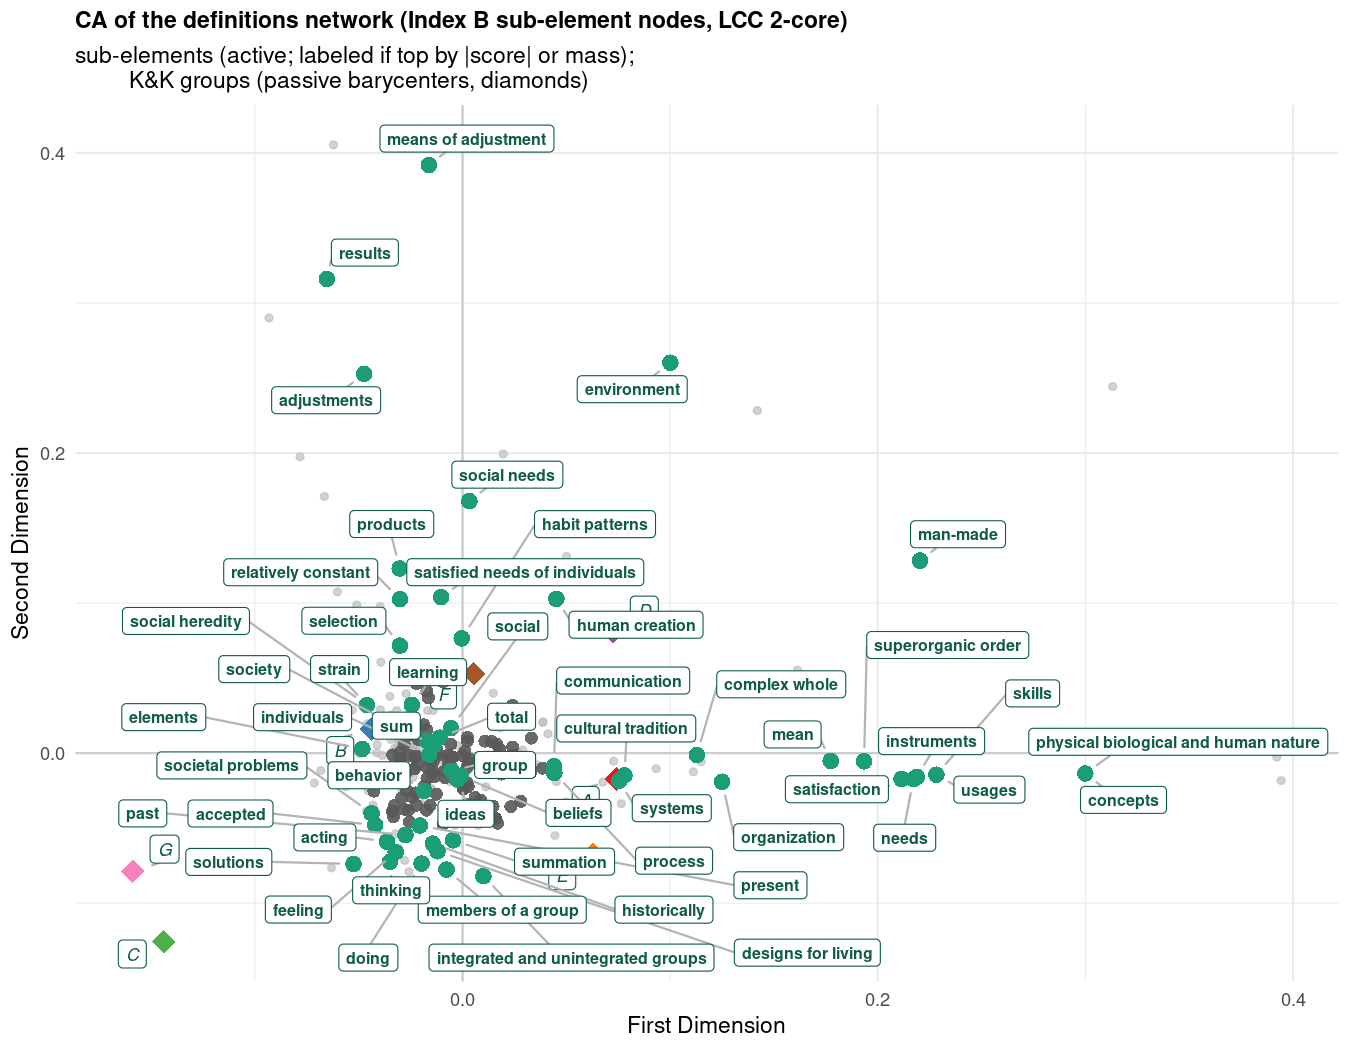
\includegraphics[width=0.85\textwidth]{figures/kk-index-b/definitions/ca-lcc2core-d12.png}
\caption{CA of the definitions network, dimensions 1 vs 2. Sub-elements are active (labelled if top by score or mass); K\&K groups are passive barycenters.}
\label{fig:ca-def}
\end{figure}

\begin{figure}[ht]
\centering
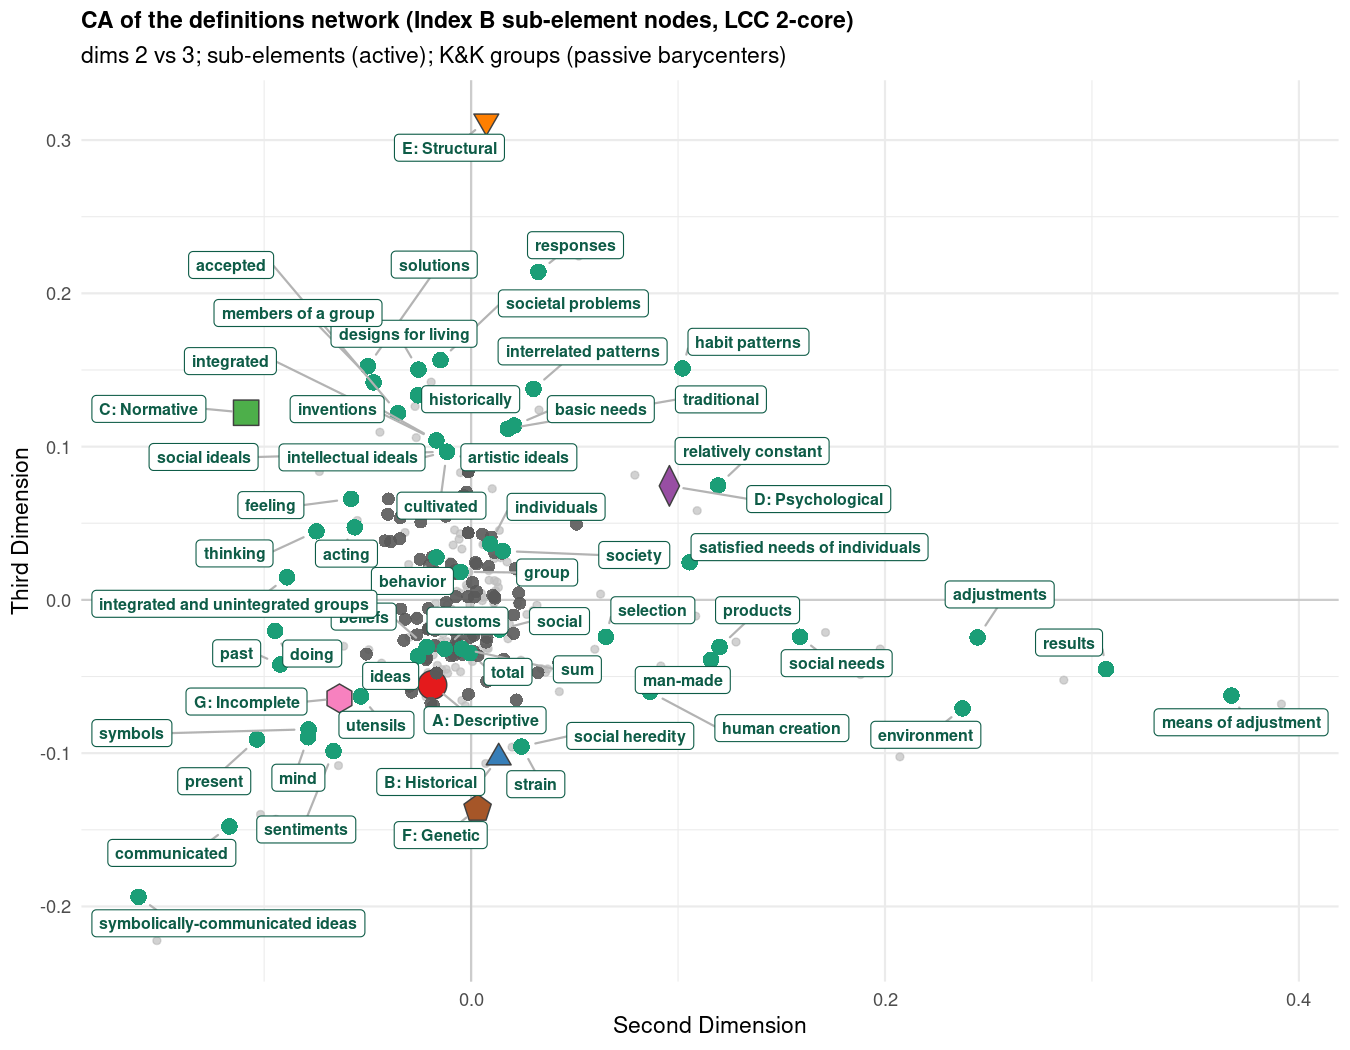
\includegraphics[width=0.7\textwidth]{figures/kk-index-b/definitions/ca-lcc2core-d23.png}
\caption{CA of the definitions network, dimensions 2 vs 3.}
\label{fig:ca-def-d23}
\end{figure}

\begin{figure}[ht]
\centering
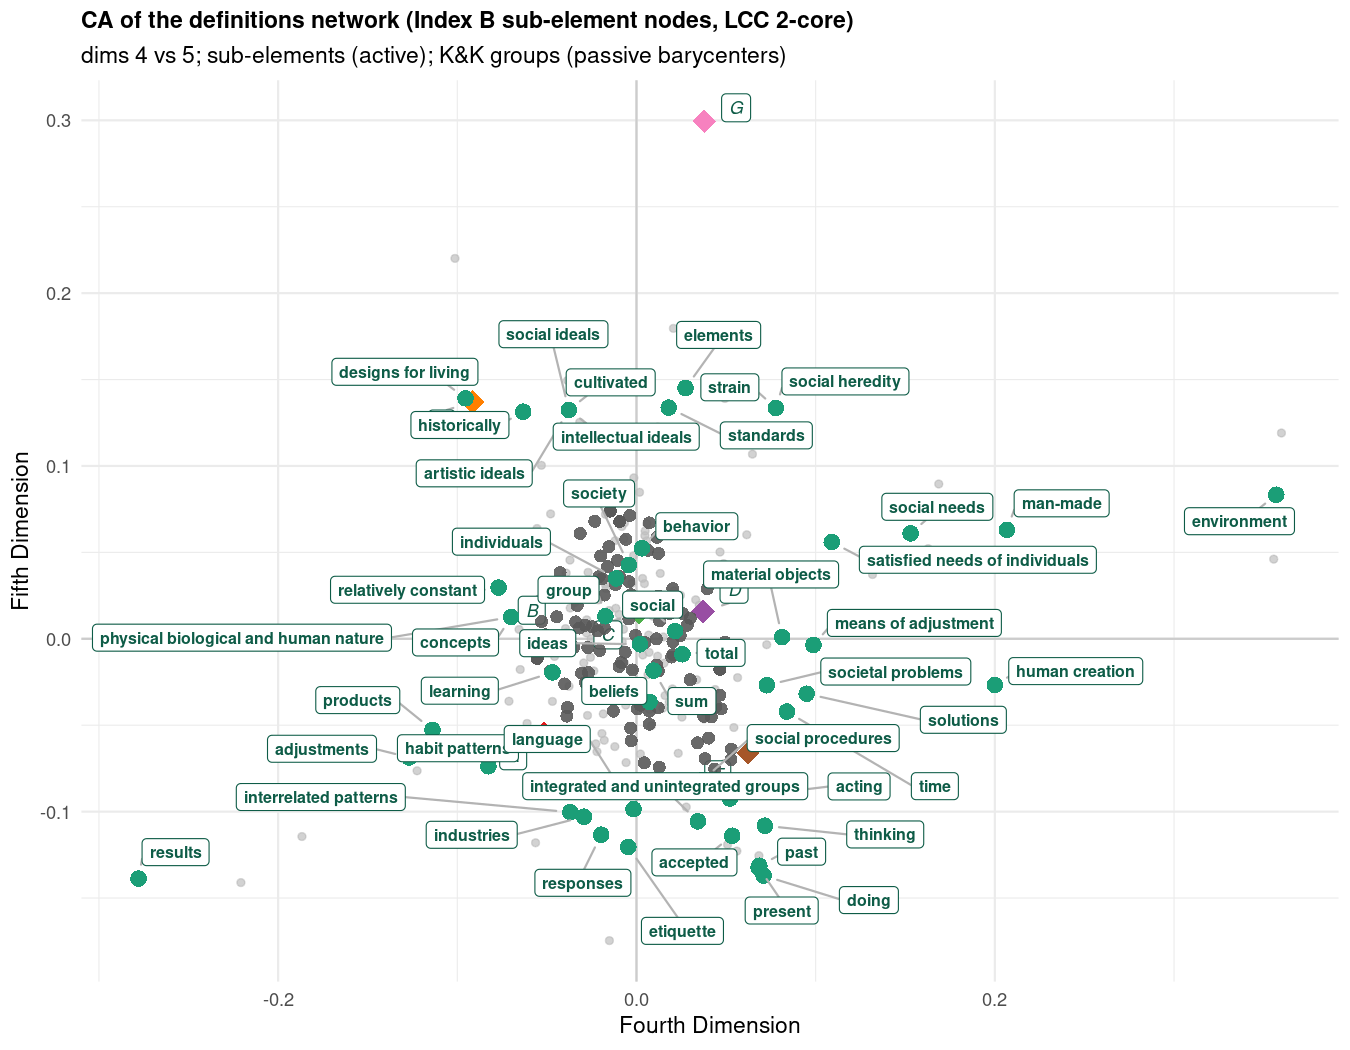
\includegraphics[width=0.7\textwidth]{figures/kk-index-b/definitions/ca-lcc2core-d45.png}
\caption{CA of the definitions network, dimensions 4 vs 5.}
\label{fig:ca-def-d45}
\end{figure}

\paragraph{Works network.} The works 2-core has 119 works, 157 sub-elements, and 845 edges. Total inertia is 20.57, with the first dimension at 2.7\% and the first five at 12.8\%. Works are the active set in the main view (Figure~\ref{fig:ca-works}). On dimension 1, Panunzio 1939 has the largest positive score, followed by White 1943 and Bernard 1942; the most negative scores go to Ford C. S. 1939, Ford C. S. 1942, and Morris 1946. The sign of each dimension is arbitrary (here the largest absolute score is positive). Those are the only dimension 1 readings offered here.

Sub-elements are the active set in the concept view (Figure~\ref{fig:ca-concepts}). The strongest positive dimension-1 scores go to ``skills'' and ``usages'' (tied at 0.16), then ``instruments,'' ``superorganic,'' and ``order.'' The most negative scores go to ``responses'' (about $-0.16$), ``societal problems,'' and ``solutions.''

\begin{figure}[ht]
\centering
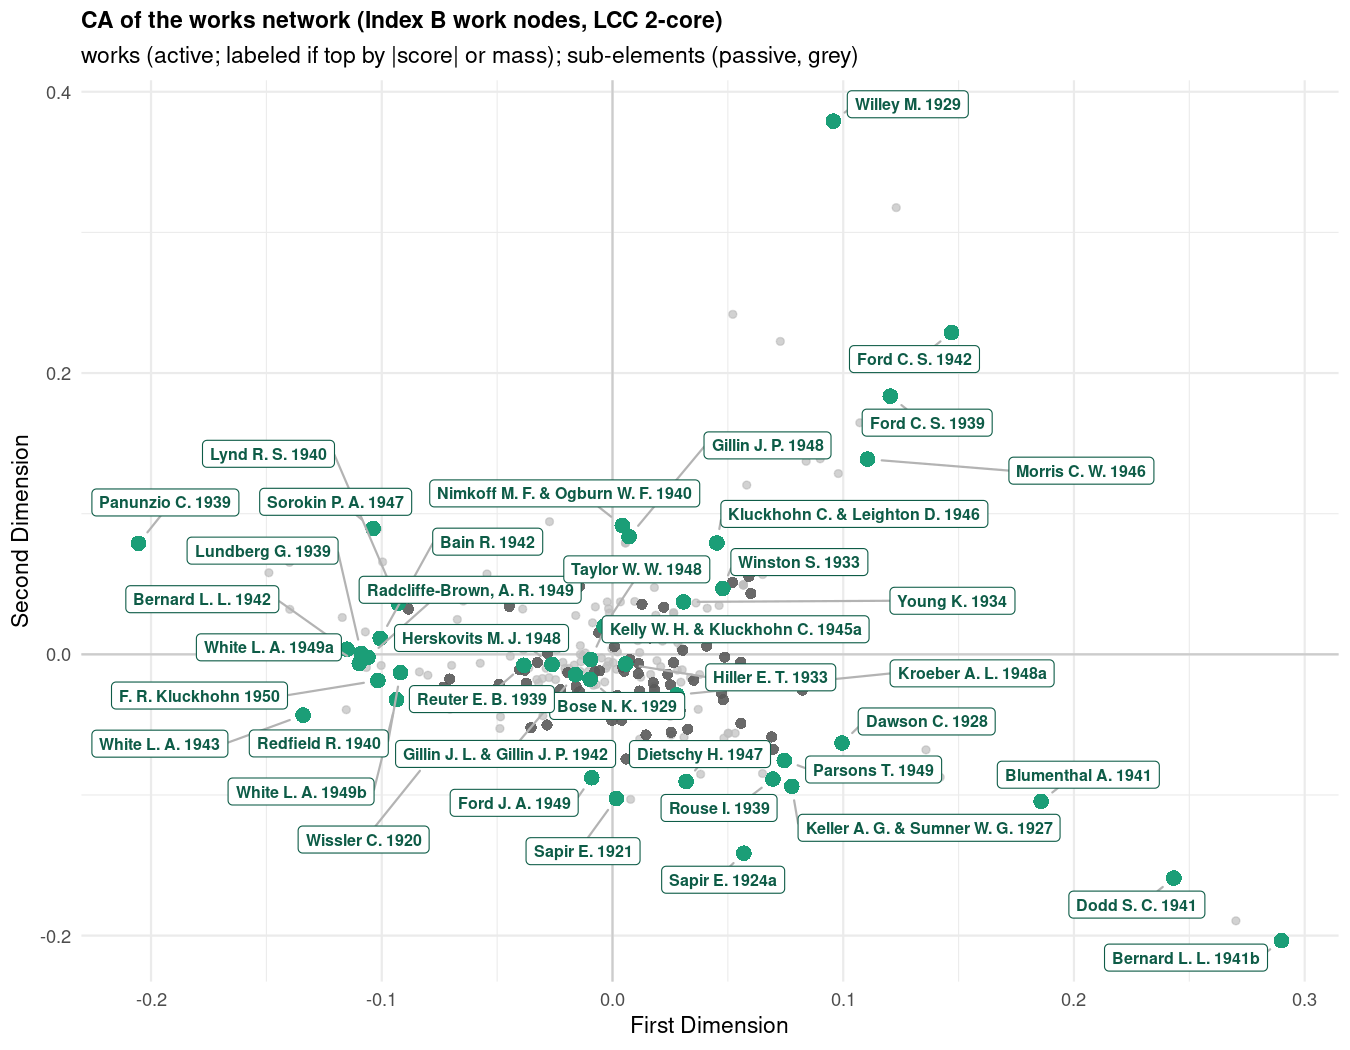
\includegraphics[width=0.8\textwidth]{figures/kk-index-b/works/ca-lcc2core-d12.png}
\caption{CA of the works network, works active, dimensions 1 vs 2.}
\label{fig:ca-works}
\end{figure}

\begin{figure}[ht]
\centering
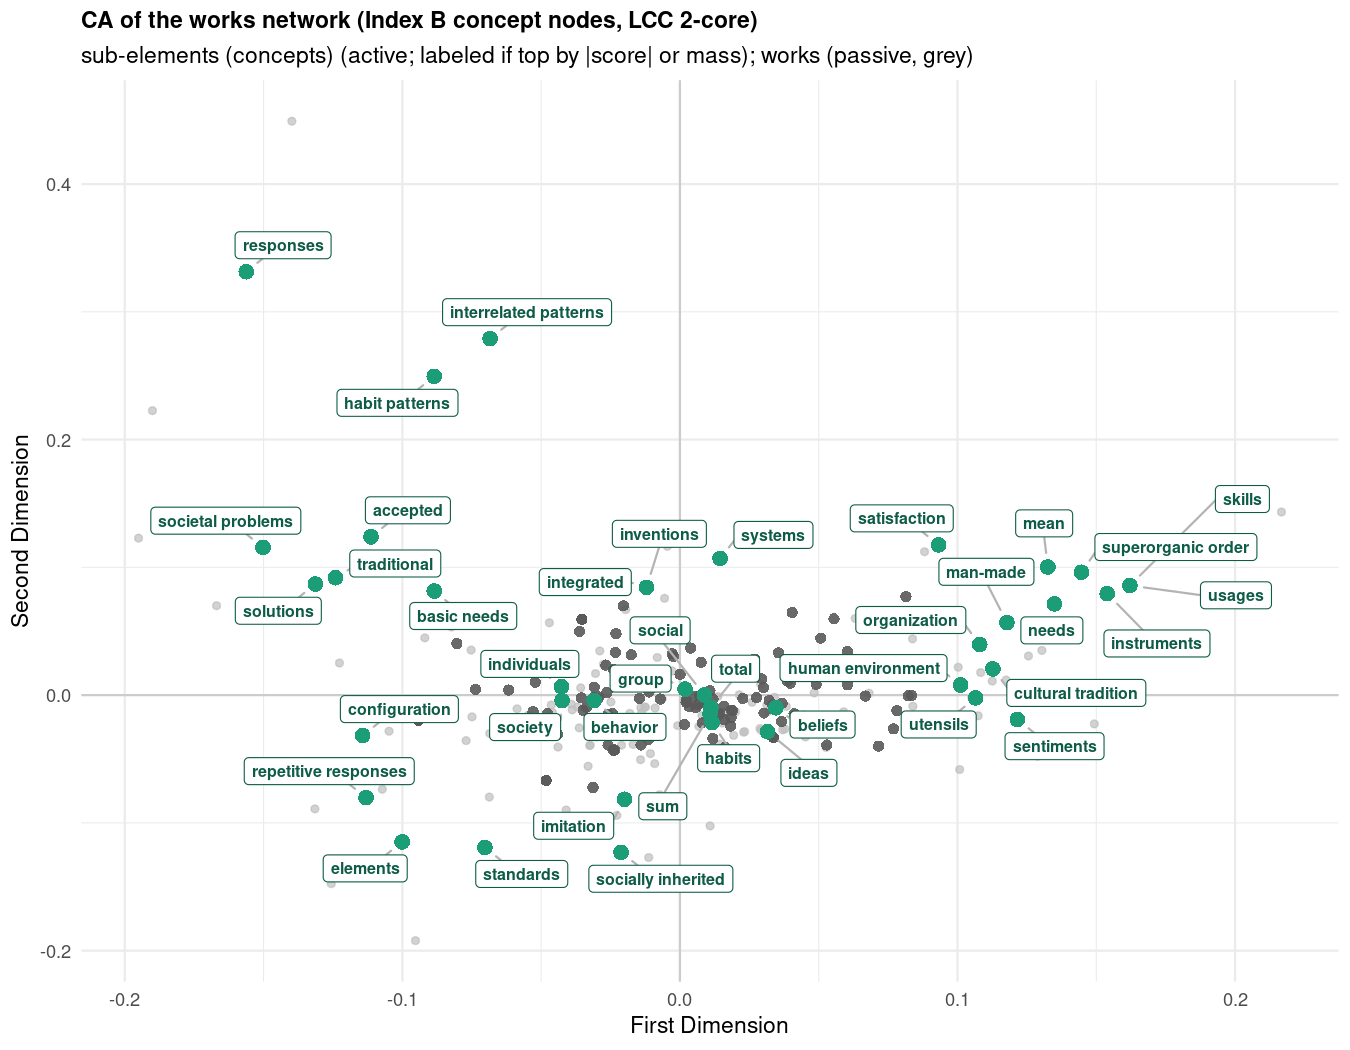
\includegraphics[width=0.8\textwidth]{figures/kk-index-b/works/ca-concepts-lcc2core-d12.png}
\caption{CA of the works network, sub-elements (concepts) active, dimensions 1 vs 2.}
\label{fig:ca-concepts}
\end{figure}

\section{Maximum spanning trees}

For each one-mode projection, ties are weighted by the number of shared neighbours, and the maximum spanning tree is the minimum spanning tree on negated weights (Kruskal's algorithm). The definitions trees use the largest component's 2-core; the works trees use the 2-core of the works network's largest component, as the definitions trees do. Node size is betweenness in the tree, and colour is the leading-eigenvector community computed on the tree.

\paragraph{Definitions network.} The code-level tree has 144 edges (of 144 possible). Its highest-betweenness codes are F-I-3 (Folsom 1931), C-I-6 (Gillin \& Gillin 1942), F-I-8 (Reuter 1939), F-II-8 (Taylor 1948), and F-I-19 (Murdock 1949a). The sub-element tree has 158 edges (of 158 possible) and its highest-betweenness sub-elements are ``social,'' ``group,'' ``society,'' ``behavior,'' and ``customs.'' Figures~\ref{fig:mst-def-code} and~\ref{fig:mst-def-sub} show the two trees.

\begin{figure}[ht]
\centering
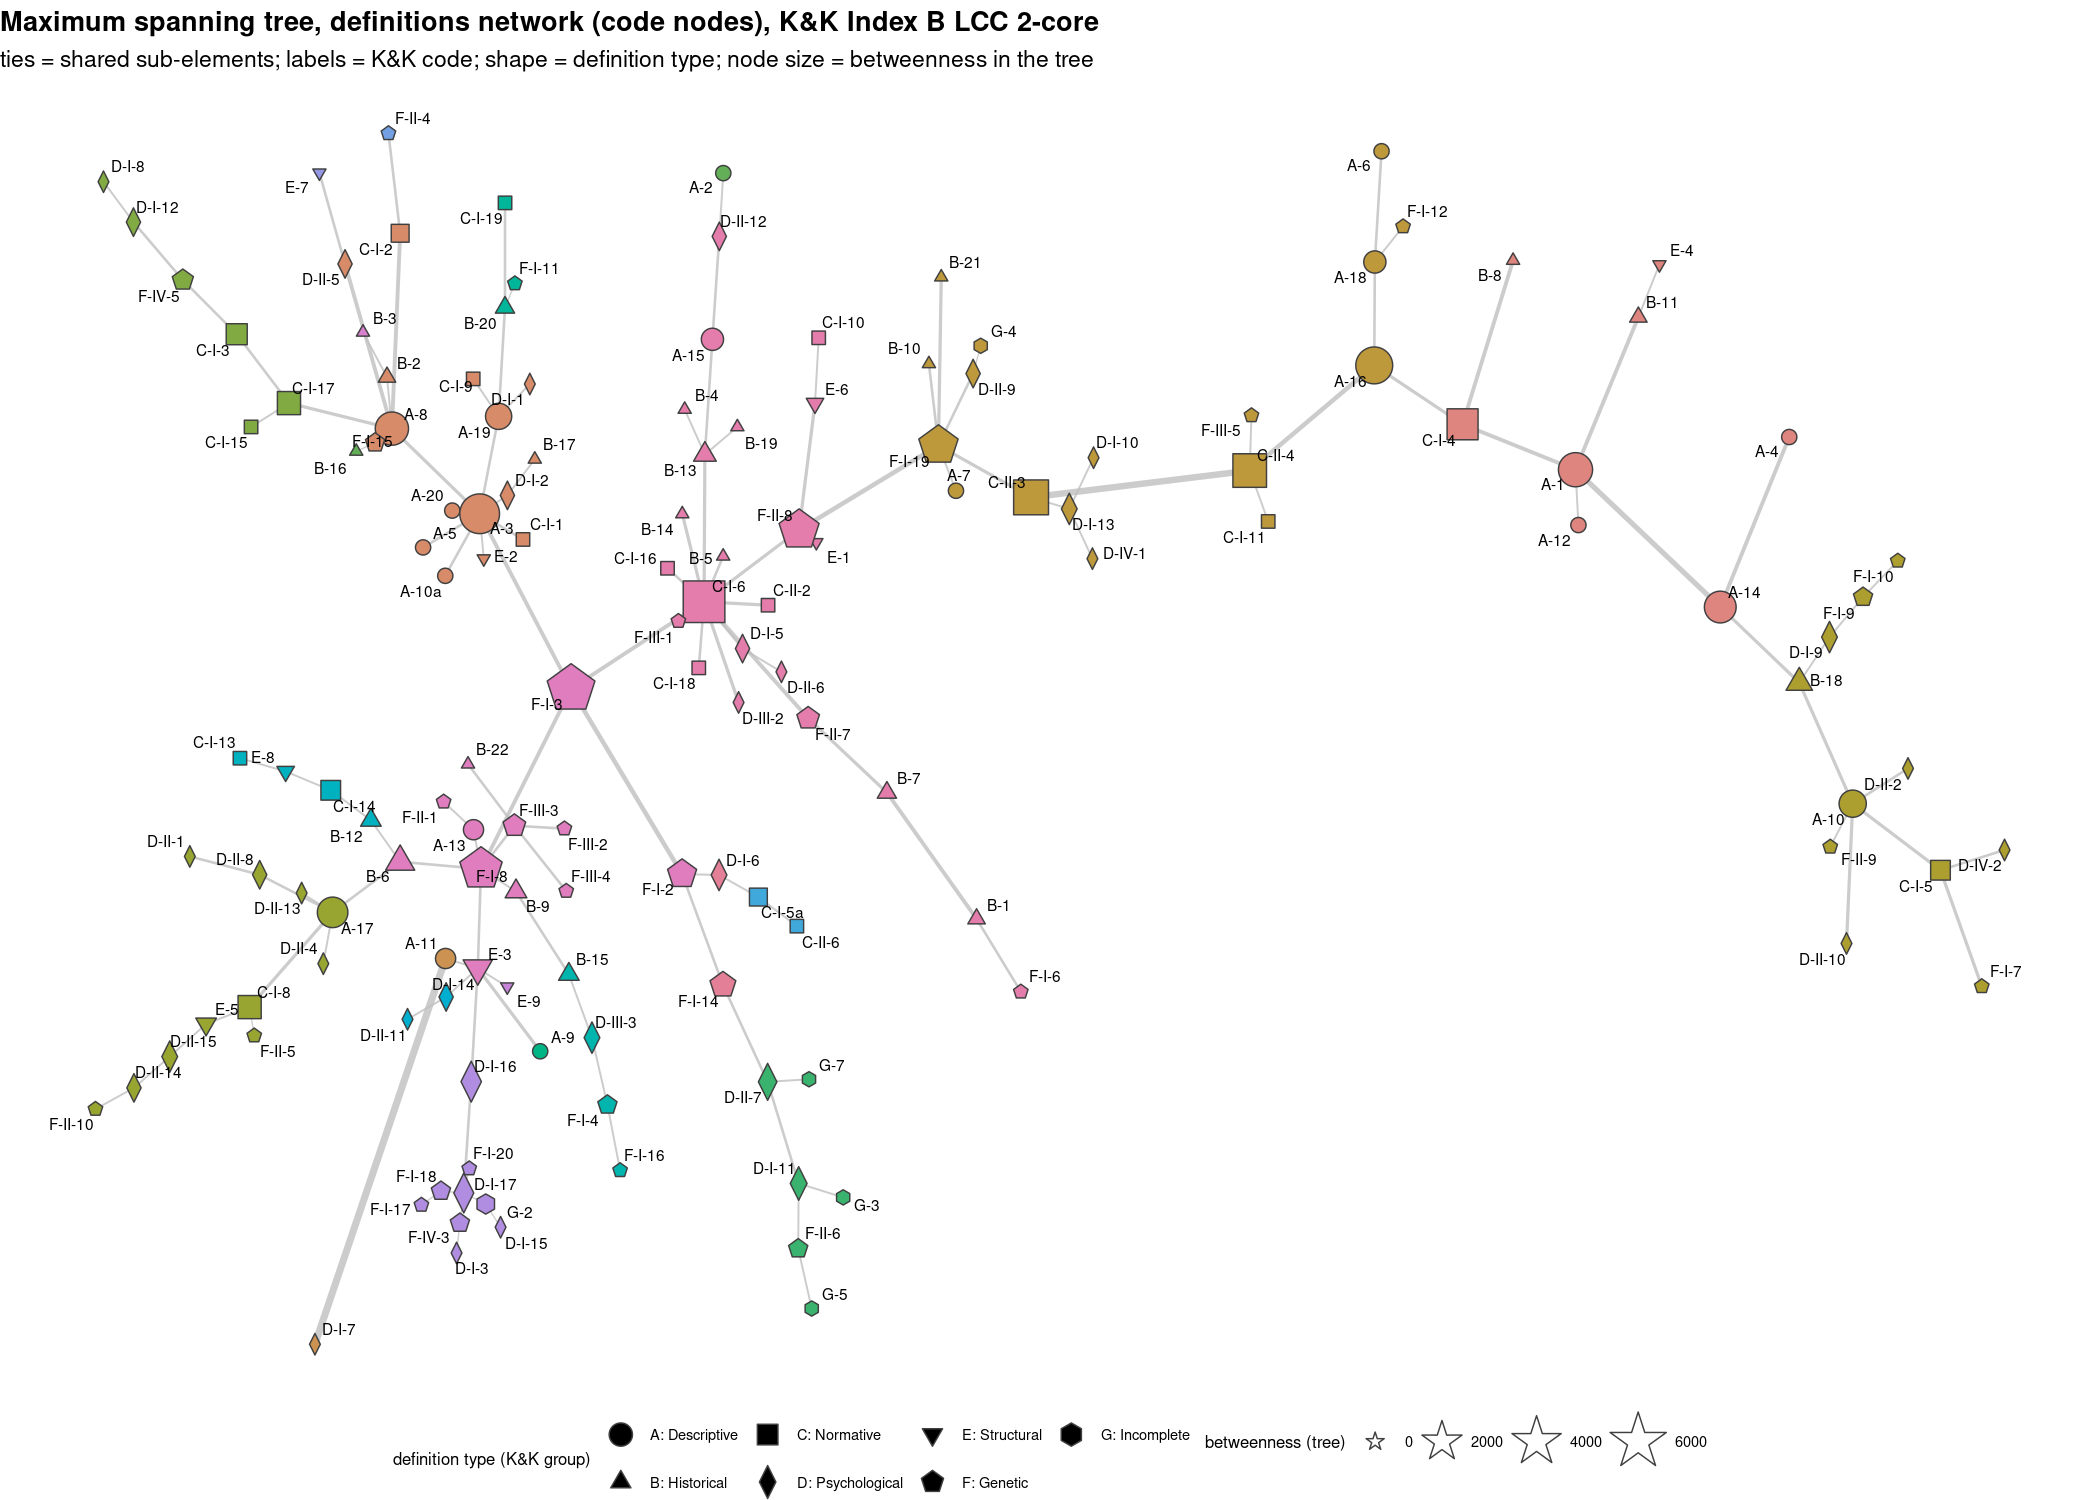
\includegraphics[width=\textwidth]{figures/kk-index-b/definitions/mst-code-comm-tree.png}
\caption{Maximum spanning tree of the definitions network, code nodes. Colour is the leading-eigenvector community on the tree; size is betweenness in the tree.}
\label{fig:mst-def-code}
\end{figure}

\begin{figure}[ht]
\centering
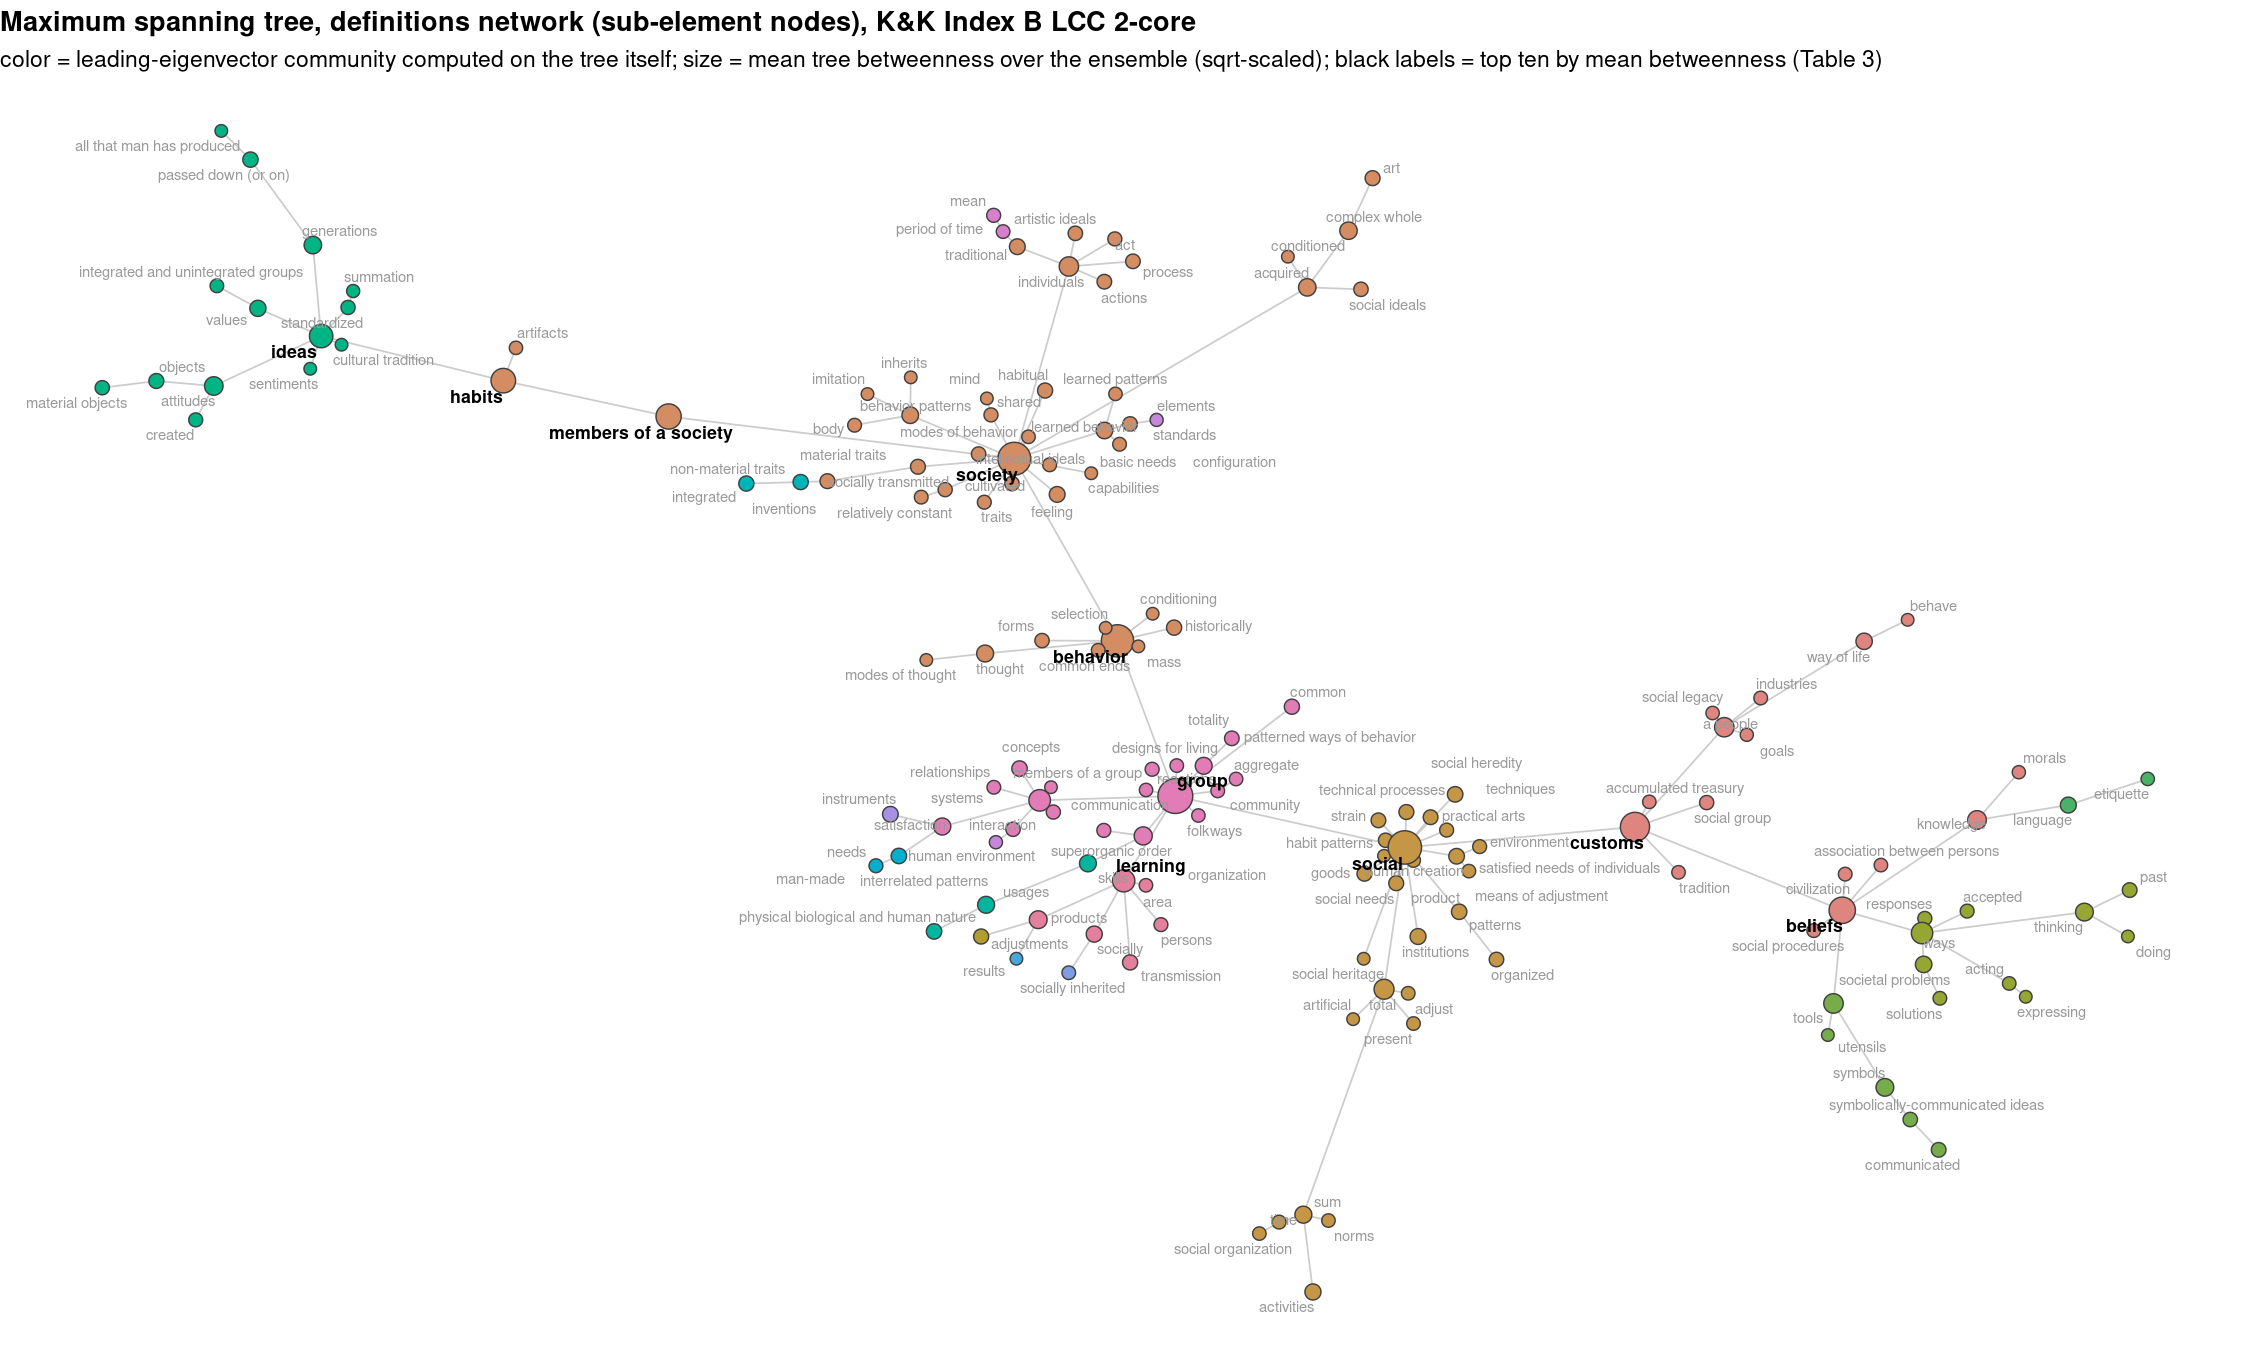
\includegraphics[width=\textwidth]{figures/kk-index-b/definitions/mst-subelement-comm-tree.png}
\caption{Maximum spanning tree of the definitions network, sub-element nodes.}
\label{fig:mst-def-sub}
\end{figure}

\paragraph{Works network.} The work-level tree has 118 edges (of 118 possible). Its highest-betweenness works are Kelly \& Kluckhohn 1945a, Young 1934, Gillin \& Gillin 1942, Winston 1933, and Kroeber 1948a. The sub-element tree has 156 edges (of 156 possible). Figures~\ref{fig:mst-works-work} and~\ref{fig:mst-works-sub} show the two trees.

\begin{figure}[ht]
\centering
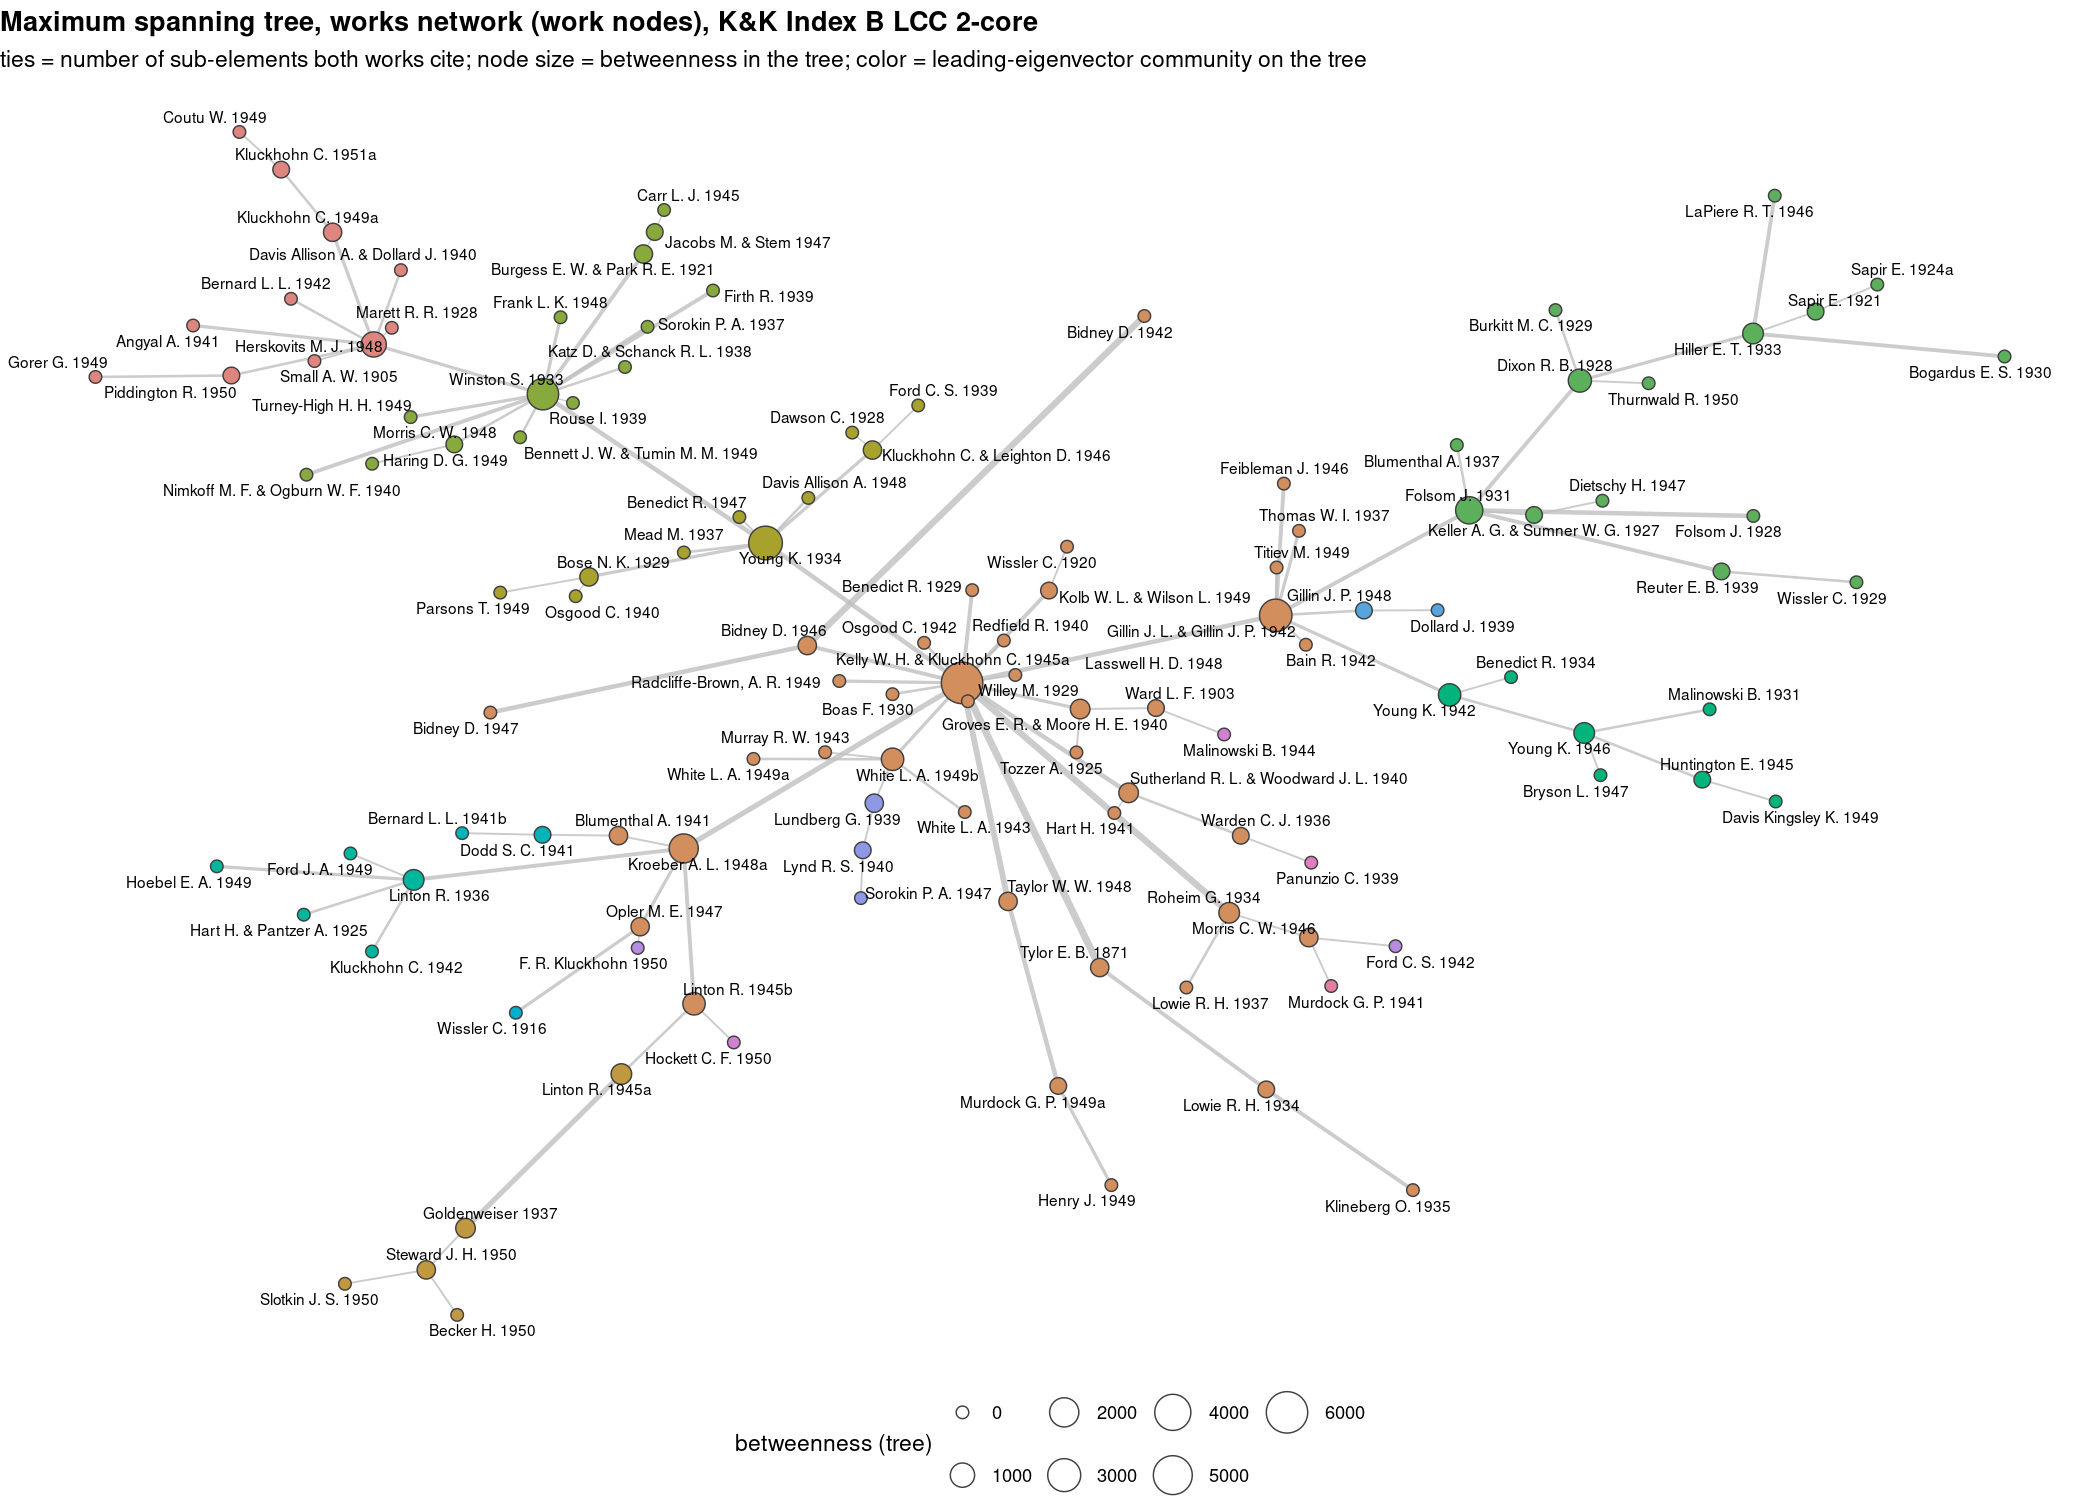
\includegraphics[width=\textwidth]{figures/kk-index-b/works/mst-work.png}
\caption{Maximum spanning tree of the works network, work nodes.}
\label{fig:mst-works-work}
\end{figure}

\begin{figure}[ht]
\centering
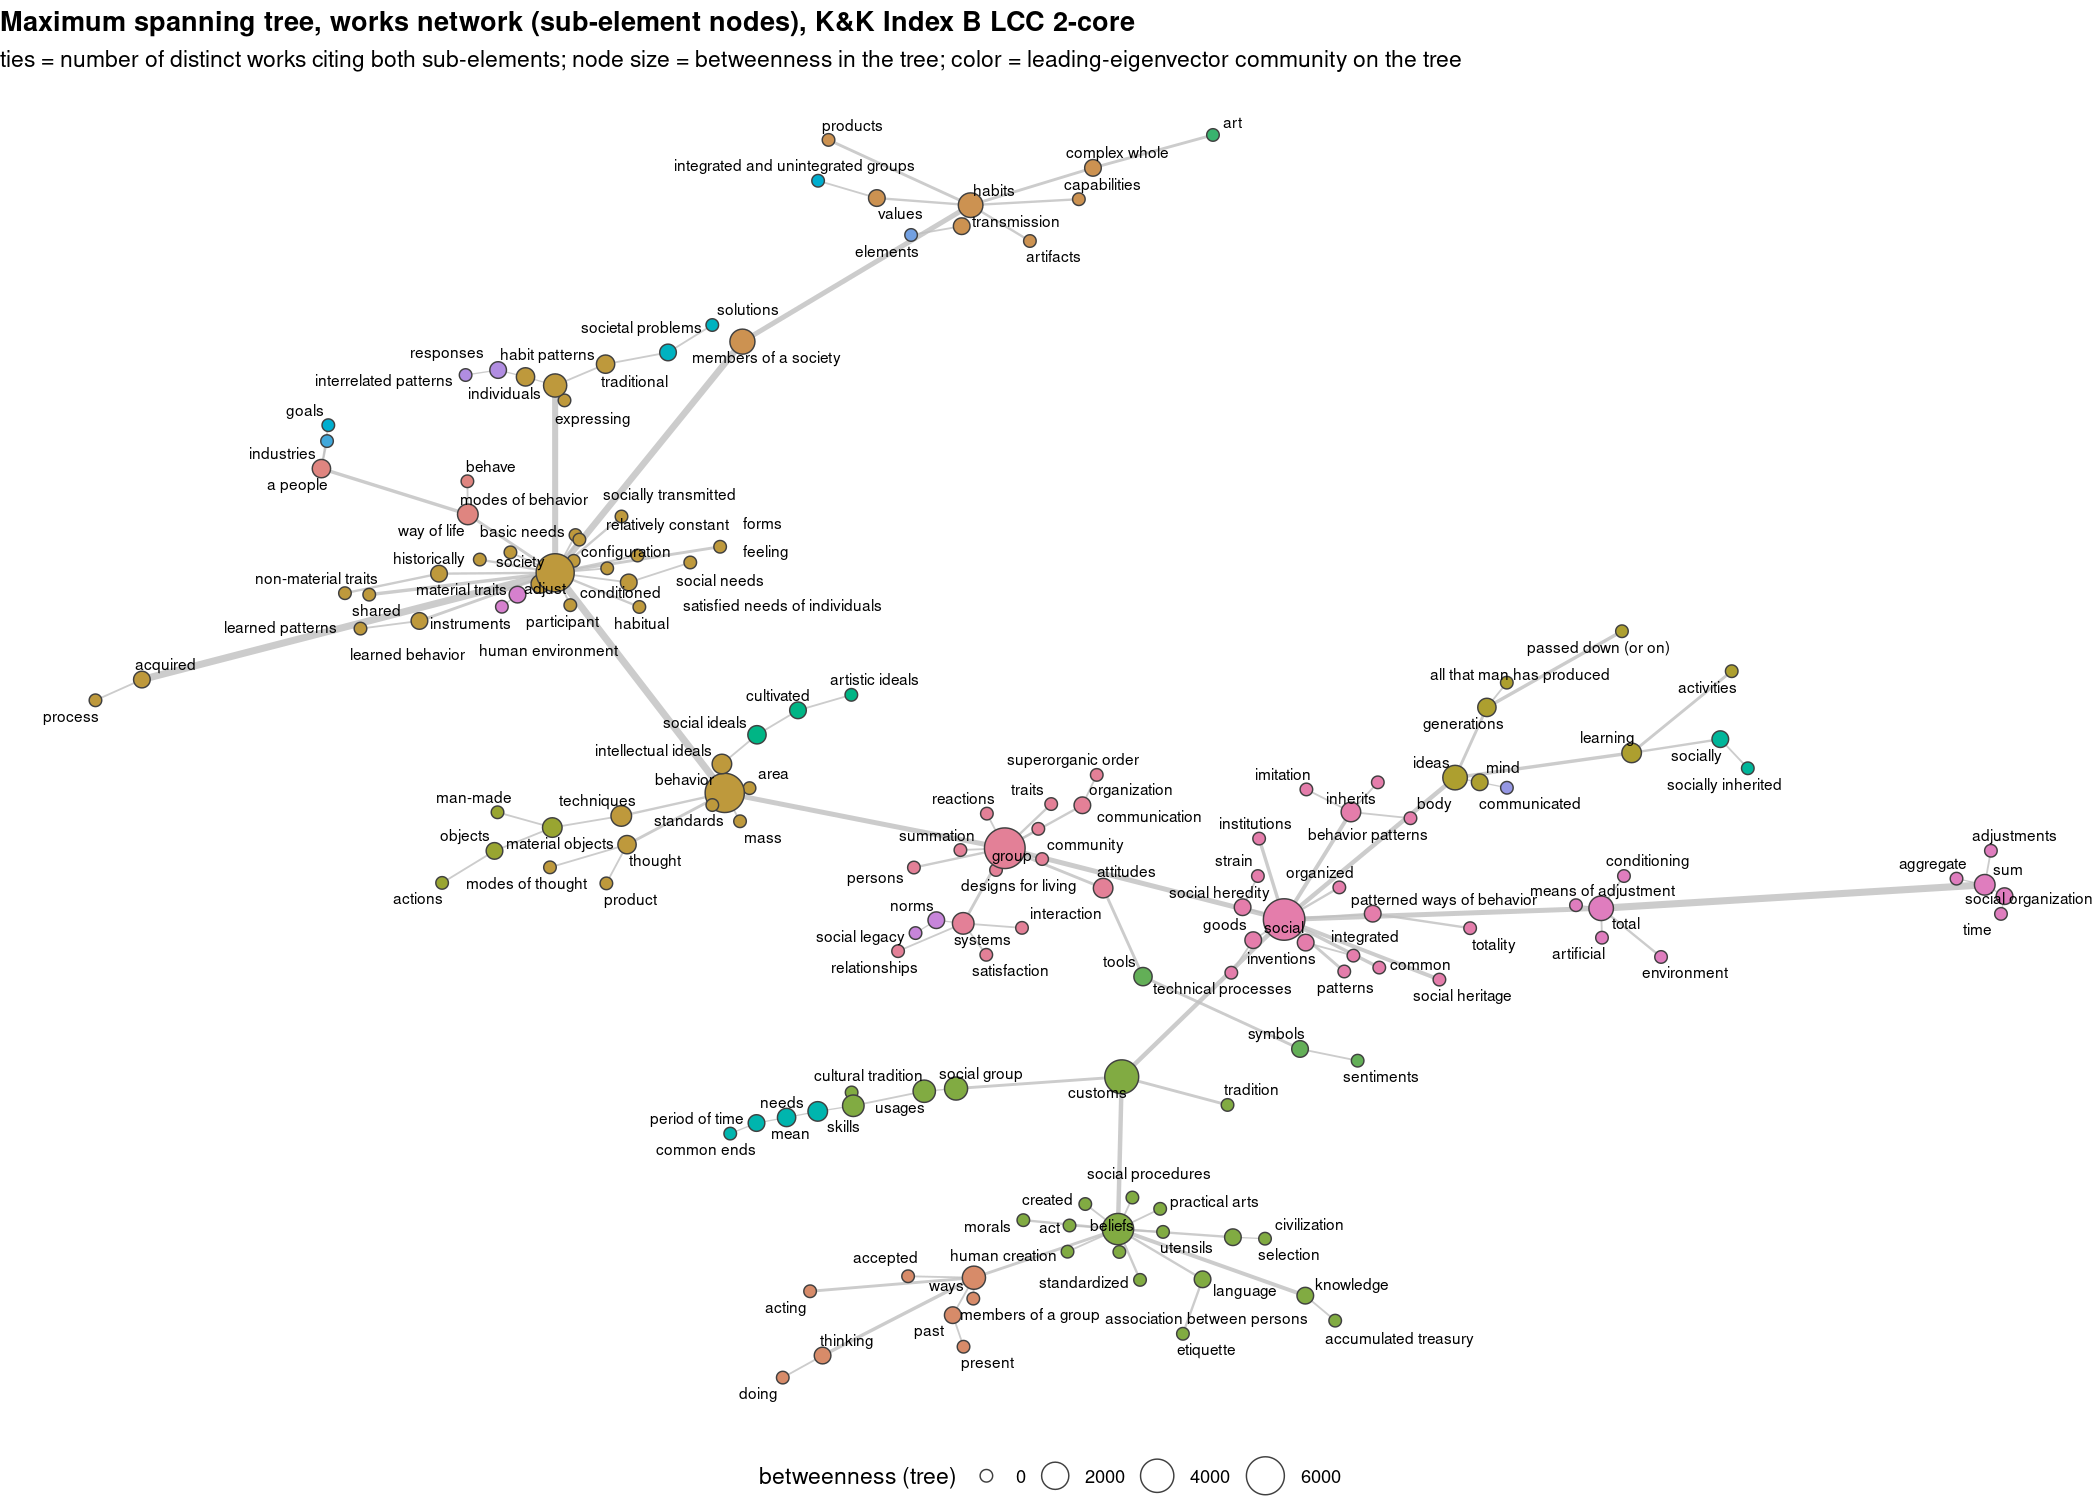
\includegraphics[width=\textwidth]{figures/kk-index-b/works/mst-subelement.png}
\caption{Maximum spanning tree of the works network, sub-element nodes. Ties count the works that cite both sub-elements.}
\label{fig:mst-works-sub}
\end{figure}

\section{Closeness and betweenness}

Closeness and betweenness are computed on each network's largest connected component, since both need connected networks. The definitions component is the largest component of the verified network (624 nodes); the works network's largest component has 593 nodes. Closeness uses the two-mode normalization $n_Y + 2(n_X - 1)$, where $n_X$ is the node's own set and $n_Y$ the other set. Betweenness uses the two-mode normalization for the larger and smaller sets, as given by Borgatti and Everett (1997). In both networks the sub-elements are the larger set. Betweenness is reported as a percentage of its normalization maximum.

\begin{table}[ht]
\centering
\caption{Most central sub-elements by closeness (top six in each network), plus the highest-closeness second-mode node, with betweenness as a percentage of the normalization maximum.}
\label{tab:centrality}
\begin{tabular}{llrrr}
\toprule
Network & Node & Degree & Closeness & Betweenness (\%) \\
\midrule
Definitions & social & 36 & 0.567 & 23.8 \\
 & society & 30 & 0.538 & 15.5 \\
 & beliefs & 18 & 0.528 & 8.1 \\
 & group & 26 & 0.528 & 10.9 \\
 & total & 22 & 0.520 & 9.8 \\
 & behavior & 24 & 0.518 & 9.6 \\
 & C-I-6 (highest-closeness code) & 19 & 0.409 & 5.1 \\
\midrule
Works & social & 33 & 0.597 & 21.8 \\
 & society & 30 & 0.590 & 14.9 \\
 & beliefs & 19 & 0.574 & 10.9 \\
 & group & 24 & 0.572 & 11.3 \\
 & behavior & 23 & 0.571 & 9.5 \\
 & ideas & 23 & 0.554 & 9.4 \\
 & Kelly \& Kluckhohn 1945a (highest-closeness work) & 51 & 0.426 & 14.3 \\
\bottomrule
\end{tabular}
\end{table}

Within the definitions network, social, society, group, and behavior rank high on both closeness and betweenness. Social has the highest betweenness among the top-closeness sub-elements in both networks; we have not checked it against every node. The highest-closeness code is C-I-6 (closeness 0.409), and the highest-closeness work is Kelly \& Kluckhohn 1945a (0.426), which also has the highest betweenness of any work (14.3\%). Full tables are in \texttt{data/kk-index-b-centrality-definitions.csv} and \texttt{data/kk-index-b-centrality-works.csv}. Closeness follows degree only loosely: beliefs (degree 18) ranks above total (degree 22). We have not measured the correlation between closeness and degree across all nodes.

\section{Not carried over from the earlier report}

The earlier report on the Boroch network also included status and prestige (HITS, PageRank, BGRM, BiRank), averages by definition type, and a provenance section. These are not repeated here. The averages and provenance sections were specific to Boroch's definition attributes.

\section{Limitations}

The networks depend on the K\&K Index B transcription and on the verified-code filter. Element names are not unique across headings, so same-named elements are merged, which can join unrelated entries. Works are keyed by author and year, so a work with several year forms may appear twice. Several readings depend on OCR corrections recorded in the repository's manual-fix files; the validators check structure and round-trips, not the content of each edge. Three codes that are not in Index A (C-I-18a, D-II-16, E-17) are included from the main text; their basis is in \texttt{data/kk-index-b-verified-extra-codes.csv}.

\end{document}
